\chapter{Realisierung}
Im diesem Kapitel geht es darum, die in der Design-Phase genannten Änderungen
praktisch umzusetzen. Dazu gehört, die einzelnen Schritte und die dabei
aufgetretenen Probleme zu erläutern. Dabei wird zuerst auf die
Benchmark-Werkzeuge und anschließend auf den Anwendungsfall eingegangen.

\section{Ausführung und Vergleich der Benchmark-Werkzeug}
Die einzelnen Benchmark-Werkzeuge und die NoSql-Systeme lassen sich nur schwer
miteinander Vergleichen, da die einzelnen Systeme sehr unterschiedliche
Funktionen bereitstellen und auch für unterschiedliche Einsatzzwecke entwickelt
wurden. So wird Memcached meist als reiner Datencache für komplette Webseiten
oder von Teilwebseiten benutzt. Während dessen ist Voldemort eher ein
Datenspeicher wie Amazons DynamoDB, Amazons S3 oder MongoDB. Dies zeigt sich
daran, dass es in Memcached und Redis sehr einfach ist einen bestehenden
Schlüssel mit einem neuen Wert abzuspeichern. Bei Voldemort ist dies nicht
einfach möglich, da bei Voldemort die einzelnen Services bzw. Server nicht
unabhängig sind. Wie auch schon in den theoretischen Grundlagen genannt wurde.
In der Regel werden in einem Cluster mehrere Versionen zu einem Schlüssel
vorhanden sein. Einige Server haben noch die alte Version, während andere Server
schon die aktuellste Version haben.

Auch spielen die unterschiedlichen Datenspeicher eine Rolle. Redis ist als
einziges System in der Lage Listen, Mengen direkt zu speichern und zu
manipulieren. Die anderen Systeme müssen den Umweg über Transformationen gehen.
Also zum Beispiel die zu speichernden Werte in JSON umwandeln und diesen dann
abspeichern. Deshalb haben die einzelnen Bechmark-Werkzeuge auch unterschiedliche
Test-Methoden.

Ein weiteres Problem sind die verschiedenen Einstellungsmöglichkeiten der
verschiedenen Tools. Die Werkzeuge Redis und Memcached erlauben eine Vielzahl
an Einstellungen vorzunehmen, wie Anzahl der Clients und Requests, Anzahl der
Datengröße. Dies ist bei Voldemort nicht möglich. Dort lässt sich nur die Anzahl
der Threads, welche die Clients darstellen, ändern. 

Die Ergebnisse der Benchmarktests sind für Redis in \ref{bench:Redis}, für
Memcached in \ref{bench:Memcached} und für Voldemort in \ref{bench:Voldemort}
dargestellt. Für Memcached und Redis sind dabei die selben Basiseinstellungen
genutzt worden. Bei Voldemort ist dies nicht möglich, da es eine andere
Konfiguration bestitzt, wie schon erwähnt wurde. 

\begin{minipage}{\linewidth}
\lstinputlisting[caption={Redis-Benchmark},label={bench:Redis}]{bench/redis-benchmark.txt}
\end{minipage}

\begin{minipage}{\linewidth}
\lstinputlisting[caption={Memcached-Benchmark},label={bench:Memcached}]{bench/memcached-benchmark.txt}
\end{minipage}

\begin{minipage}{\linewidth}
\lstinputlisting[caption={Voldemort-Benchmark},label={bench:Voldemort}]{bench/voldemort-benchmark.txt}
\end{minipage}

Man könnte nun als Basisfall die Set- und Get-Test für Memcached und Redis
viederholen und danach vergleichen in wieweit sich beide Systeme bei
unterschiedlichen Lasten verteilen. Ob es eine Konfiguration gibt, bei der Redis
besser abschneidet als Memcached. Eine größe Einschränkung ist noch zu tätigen,
da bei den Tests sowohl das zutestende System als auch das Testwerkzeug auf ein
und derselben Maschine liefen. Dies ist für einen realen Testversuch jedoch nicht
geeigntet. Da praktisch der gesammte Netzwerkverkehr wegfällt. Außerdem ist es
nicht möglich die Last auf größere Mengen hochzustellen, da sonst entweder
das Testtool oder das System durch das Betriebssystem beeinflusst würden. Wenn
jedoch nur kleine Datenmengen benutzt werden ist der Test praktisch sofort
abgeschlossen.

\subsection{Realisierung des Benchmark-Werkzeuges}
Das Benchmark-Werkzeug wurde als C-Anwendung realisiert. Dabei wurde für die
Kommandozeile, die Bibliothek gengetops benutzt, welche es ermöglicht über eine
DSL die benötigten Optionen zu definieren und den Rest der Bibliothek zu
überlassen. Dies sorgt für eine bessere Wartbarkeit der Anwendung. Darauf hin
werden die entsprechenden Test-Methoden gestartet. Dabei besteht ein
signifikanter Unterschied zwischen dem Original und der Neuentwicklung. Beim
Original laufen die Tests sequentiell ab, zuerst wird der set-Test ausgeführt
und anschließend wird der get-Test ausgeführt. Bei redis-Benchmark, wie auch
bei der Neuentwicklung können die Tests selektiert werden. Dies setzt jedoch
voraus, dass für einzelne Tests ein Setup durchgeführt werden muss, welches
früher der vorherige Test übernommen hatte. Alle Test-Methoden benutzen auch
nicht mehr direkt den Socket, sondern die von Memcached bereitgestellte
Bibliothek.

\section{Realisierung des Anwendungsfalls}
Der Anwendungsfall wurde als Django-Projekt umgesetzt. Dazu wurde als Beispiel
ein einfacher Buch-Shop gewählt, bei dem die Benutzer die angebotenen Bücher von
0 bis 5 Sterne bewerten können und die Anwendung daraus einen Top-Liste erstellt.
Die Abbildung \ref{fig:django-start} zeigt dabei die aktuelle Startseite der
Web-Anwendung mit einer Übersicht über die Anzahl der Einträge in der Datenbank.

\begin{figure}
\centering
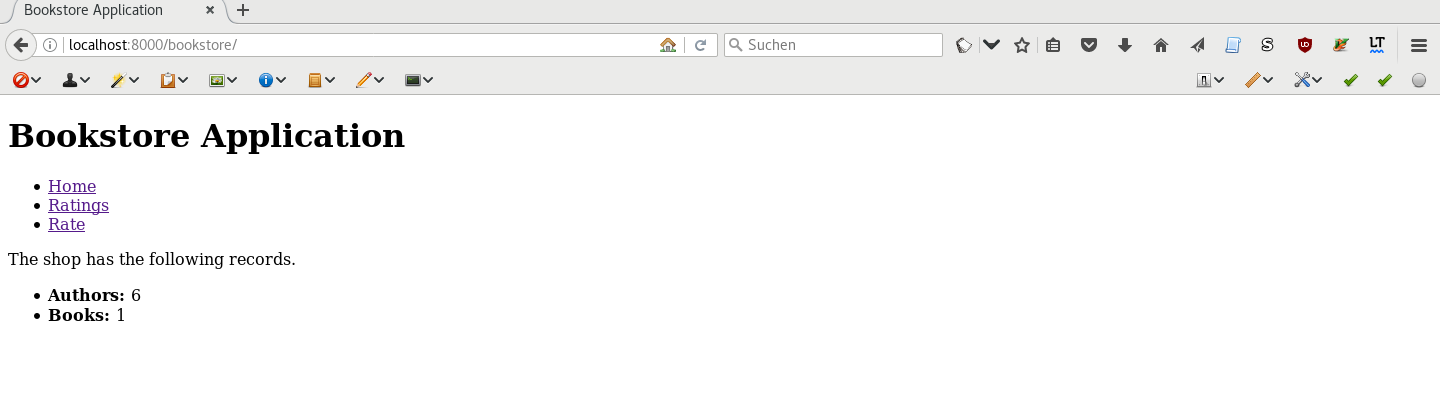
\includegraphics[scale=0.25]{images/Web-Application-Entry.png}
\caption{Web-Anwendung Startseite}
\label{fig:django-start}
\end{figure}

Derzeit gibt es zwei Benutzergruppen, welche verschiedene Bereiche der Anwendung
benutzen können. Die erste Gruppe ist die Gruppe der Administratoren, welche
Zugriff auf alle Funktionen der Anwendung haben. Die Administratoren können neue
Bücher anlegen, editieren oder löschen. Dies erfolgt über den von Django
bereitgestellte Administrator-Bereich. Der Administrator-Bereich ist eigentlich
die Admin-Anwendung. Eine Django-Anwendung ist eine spezielle Komponente, welche
genau eine Aufgabe erfüllt. Eine einmal entwickelte Anwendung sollte im
Ideal-Fall so konzipiert sein, dass sie in mehreren Django-Projekten zum Einsatz
kommen kann. In der Abbildung \ref{fig:django-create} ist die erzeugte Seite
für die Bücher dargestellt, welche vom der erwähnten Django-Admin Anwendung
erzeugt wurde.

Ein Django-Projekt besteht dabei zwingend aus mindestens einer
Django-Anwendung. Die Admin-Anwendung erzeugt dabei, für einmal definierte
Modelle, selbständig Oberflächen um die CRUD-Methoden bereitzustellen.

\begin{figure}
\centering
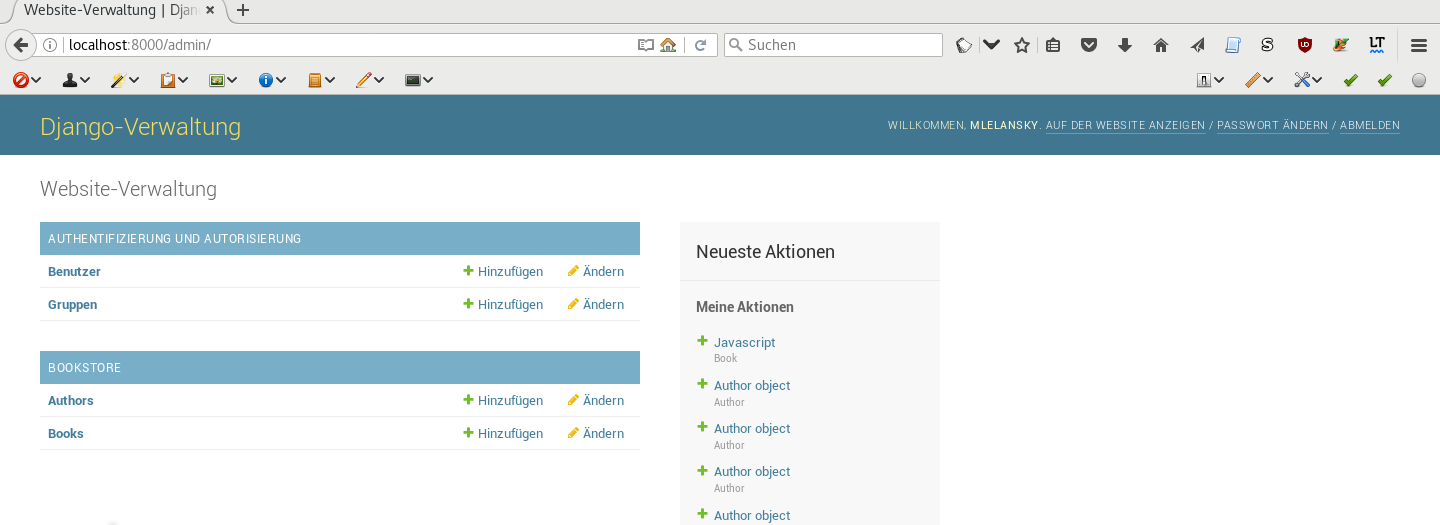
\includegraphics[scale=0.25]{images/Creation.png}
\caption{Büchererzeugung}
\label{fig:django-create}
\end{figure}

Die zweite Gruppe ist die Gruppe der normalen Benutzer, welche die eigentliche
Bewertung vornehmen können. Diese können aus einer Liste von registrierten
Büchern ein Buch auswählen und die dazugehörige Bewertung vornehmen. Die
Abbildung \ref{fig:django-rate} zeigt dabei die Formularseite, wo die Benutzer 
abstimmen können. Die Ergebnisseseite ist in der Abbildung \ref{fig:django-list}
dargestellt.

\begin{figure}
\centering
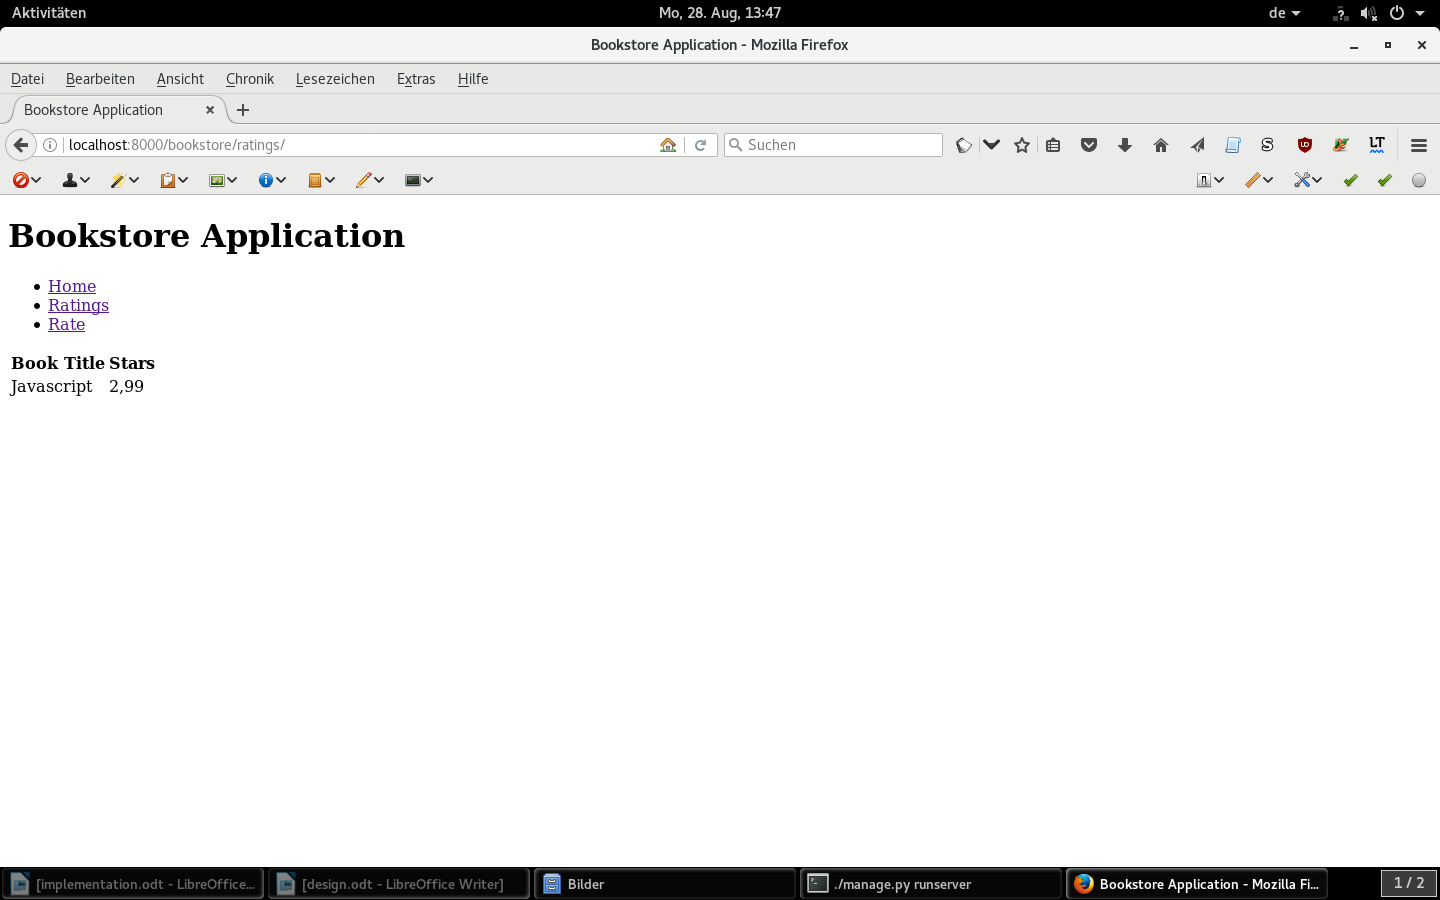
\includegraphics[scale=0.25]{images/Ratings.png}
\caption{Top-Liste}
\label{fig:django-list}
\end{figure}

\begin{figure}
\centering
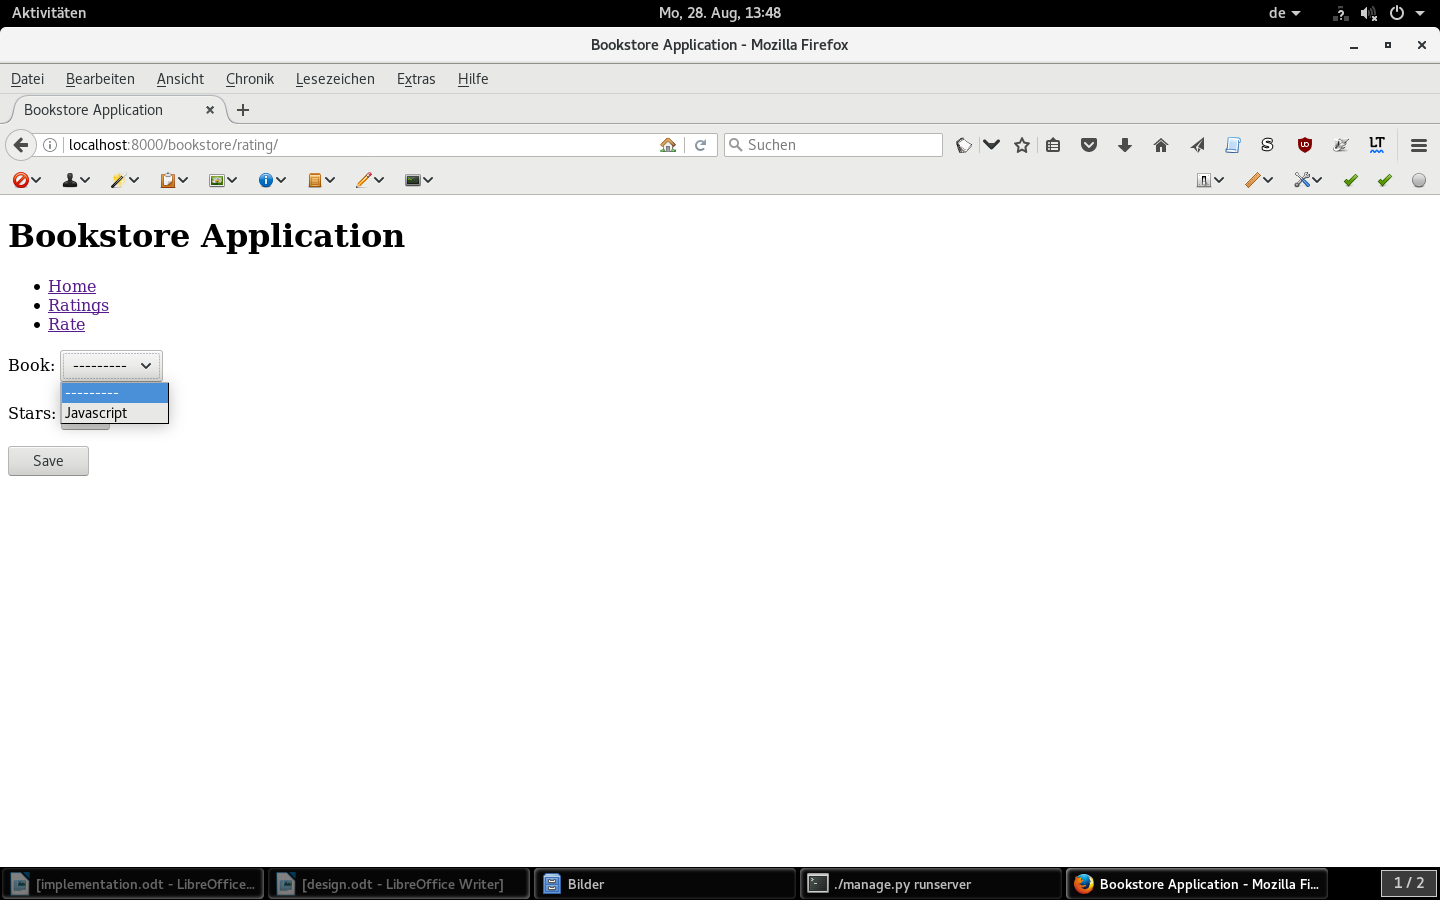
\includegraphics[scale=0.25]{images/Rating.png}
\caption{Rating von Büchern}
\label{fig:django-rate}
\end{figure}

Zusätzlich wurde noch ein Django-Kommando definiert um schnell viele Abstimmungen
vorzunehmen zu lassen.

\subsection{Anbindung der NoSql-Systeme}
Wie schon in der Design-Phase erwähnt, existiert für Memcached bereits eine
Django-Implementierung und auch die benötigten Client-Bibliotheken. Diese wurden
einfach in die bestehende Anwendung integriert, in dem die benötigten
Konfigurationseinstellungen vorgenommen wurden. Dabei wurde zusätzlich die Hilfe
der Bibliothek django-configurations\footnote{\url{https://pypi.python.org/pypi/django-configurations/2.0}}
benutzt um über einfache Optionsschalter die jeweiligen Cache"=Implementierungen
auszutauschen. Die Redis-Implementierung wurde nach dem gleichen Prinzip
übernommen.

Da der Voldemort-Client nicht funktionierte, wurde wie schon beschrieben ein
neuer \gls{REST}-Client entwickelt. Der Client wird dabei mit den Rest-Endpunkten
und den Node-Ids initialisiert. Danach kann der Anwender die Methoden frei
benutzen. Ein Abmelden, wie bei den anderen Bibliotheken ist hierbei nicht
notwendig, da alle Verbindungen über das HTTP-Protokoll laufen und nicht direkt
über Sockets. Danach wurde der neue Voldemort-Cache implementiert. Dabei wurde
die Django-Cache-Implementierung für Memcached als Ausgangsbasis genommen, da
von der API her Memcached und Voldemort ähnlich sind im Gegensatz zu Redis.

Bei der Anwendung sind alle Systeme gleich gut benutzbar. Je nach Anwendungsfall
kann man mehr oder weniger Aktionen von Django übernehmen lassen. Der einfachste
Fall ist Django die Speicherung der kompletten Anwendung zu überlassen. Etwas
mehr Kontrolle bekommt man, wenn man die Seiten, welche gespeichert werden
sollen selbst festlegt. Nochmals mehr Kontrolle erlangt man, wenn man nur Teile
einer Seite zwischenspeichert und die volle Kontrolle bekommt man, wenn man die
Zugriffsmethoden direkt verwendet. Diese Entscheidung muss jedoch jeder
Entwickler je nach Situation selber fällen.

\subsection{Probleme und offene Punkte bei der Umsetzung}
Trotz der erfolgreichen Anbindung von Voldemort an Django gibt es noch einige
Probleme, bzw. offene Punkte, welche man in einem weiteren
Implementierungsschritt umsetzen kann.

Das erste Problem ist die \gls{REST}-API von Voldemort, welche auch noch nicht
ganz ausgereift ist. Dies zeigt sich zum Beispiel im Verhalten mit den
Vektor-Uhren und Versionen. Außerdem kann es manchmal zu unkontrollierten
Verhalten beim  Speichern und Löschen kommen. Ein weiterer Punkt ist die Übergabe
der Serverinformationen, welche sich derzeit aus URL und Node-Id für den gesamten
Cluster zusammensetzt. Dies ist nicht wünschenswert, da normalerweise, der
Standard Java-Client und auch der rudimentäre Python-Client mit einem Server
des Clusters zufrieden sind und sich die restlichen Informationen vom Cluster
holen. Die normale REST-API bietet jedoch keine Möglichkeit die Metadaten des
Clusters abzufragen. Um die Metadaten des Clusters zu bekommen, muss erst der
existierende Koordinator-Service gestartet werden, welcher dann auch das
komplette Routing übernimmt.

Die Anwendung verfügt derzeit auch über keine Benutzerregistrierung, dies ist
aber notwendig um zu verhindern, dass jemand einen Artikel mehrfach bewertet.

Derzeit ist die entwickelte Anwendung nicht wie eine typische Django-Anwendung
wiederverwendbar, da die Domäne und das Abstimmungssystem in einer Anwendung sind.
Eine Verbesserung wäre es, wenn man das Abstimmungssystem unabhängig von den
einzelnen Produkten ist. Dazu müsste man die derzeitige Abhängigkeit in der
Tabelle zu den Produkten aufheben und die Information, für welches Produkt
abgestimmt wurde, redundant mit speichern.
